\documentclass[a4paper,11pt]{article}

\usepackage{clrscode}

\usepackage{geometry}
\geometry{
 a4paper,
 left=30mm,
 top=30mm,
}
\usepackage[utf8]{inputenc}

\usepackage{graphicx}
\usepackage[english]{babel}
\usepackage{color}
\usepackage[dvipsnames]{xcolor}
\usepackage[colorlinks=true,urlcolor=blue,citecolor=black]{hyperref}
\usepackage{url}
%\urlstyle{same}
%\urlstyle{rm}
\urlstyle{sf}
%\urlstyle{tt}
\usepackage[font=footnotesize,labelfont=bf]{caption}
\usepackage[labelfont=it,textfont={it},singlelinecheck=on,justification=centering]{caption}
%full name for appendix
\usepackage[title]{appendix}
\usepackage{float}
\setlength{\parindent}{2em}
\usepackage{parskip}
%for code
\usepackage{listings}
%for math
\usepackage{amsmath}
\usepackage{breqn}
\usepackage{pdfpages}
\linespread{1.1}
\setlength{\emergencystretch}{3em}

\usepackage{ifxetex,ifluatex}
\usepackage{etoolbox}
\usepackage{tikz}

\usepackage{framed}

%water mark
\usepackage{eso-pic}

\newcommand{\watermark}[3]{\AddToShipoutPictureBG{
	\parbox[b][\paperheight]{\paperwidth}{
		\vfill%
		\centering%
	\tikz[remember picture, overlay]%
	  \node [rotate = #1, scale = #2] at (current page.center)%
	      {\textcolor{gray!80!cyan!30}{#3}};
	  \vfill}}}
\usepackage{blindtext}
%water mark end


% conditional for xetex or luatex
\newif\ifxetexorluatex
\ifxetex
  \xetexorluatextrue
\else
  \ifluatex
    \xetexorluatextrue
  \else
    \xetexorluatexfalse
  \fi
\fi
%
\ifxetexorluatex%
  \usepackage{fontspec}
  \usepackage{libertine} % or use \setmainfont to choose any font on your system
  \newfontfamily\quotefont[Ligatures=TeX]{Linux Libertine O} % selects Libertine as the quote font
\else
  \usepackage[utf8]{inputenc}
  \usepackage[T1]{fontenc}
  \usepackage{libertine} % or any other font package
  \newcommand*\quotefont{\fontfamily{LinuxLibertineT-LF}} % selects Libertine as the quote font
\fi

\newcommand*\quotesize{60} % if quote size changes, need a way to make shifts relative
% Make commands for the quotes
\newcommand*{\openquote}
   {\tikz[remember picture,overlay,xshift=-4ex,yshift=-2.5ex]
   \node (OQ) {\quotefont\fontsize{\quotesize}{\quotesize}\selectfont``};\kern0pt}

\newcommand*{\closequote}[1]
  {\tikz[remember picture,overlay,xshift=4ex,yshift={#1}]
   \node (CQ) {\quotefont\fontsize{\quotesize}{\quotesize}\selectfont''};}

% select a colour for the shading
\definecolor{mygray}{gray}{0.95}
\colorlet{shadecolor}{mygray}

\newcommand*\shadedauthorformat{\emph} % define format for the author argument

% Now a command to allow left, right and centre alignment of the author
\newcommand*\authoralign[1]{%
  \if#1l
    \def\authorfill{}\def\quotefill{\hfill}
  \else
    \if#1r
      \def\authorfill{\hfill}\def\quotefill{}
    \else
      \if#1c
        \gdef\authorfill{\hfill}\def\quotefill{\hfill}
      \else\typeout{Invalid option}
      \fi
    \fi
  \fi}
% wrap everything in its own environment which takes one argument (author) and one optional argument
% specifying the alignment [l, r or c]
%
\newenvironment{shadequote}[2][l]%
{\authoralign{#1}
\ifblank{#2}
   {\def\shadequoteauthor{}\def\yshift{-2ex}\def\quotefill{\hfill}}
   {\def\shadequoteauthor{\par\authorfill\shadedauthorformat{#2}}\def\yshift{2ex}}
\begin{snugshade}\begin{quote}\openquote}
{\shadequoteauthor\quotefill\closequote{\yshift}\end{quote}\end{snugshade}}


\usepackage{listings}
\lstdefinestyle{myListStyle}{
  numbers=left,
  stepnumber=1,
  numbersep=10pt,
  tabsize=2,
  showspaces=false,
  showstringspaces=false
}

\usepackage[dvipsnames]{xcolor}
\usepackage{listings}

\newcommand\YAMLcolonstyle{\color{darkgray}\mdseries}
\newcommand\YAMLkeystyle{\color{black}\bfseries}
\newcommand\YAMLvaluestyle{\color{gray}\mdseries}

\makeatletter

% here is a macro expanding to the name of the language
% (handy if you decide to change it further down the road)
\newcommand\language@yaml{yaml}

\expandafter\expandafter\expandafter\lstdefinelanguage
\expandafter{\language@yaml}
{
  keywords={true,false,null,y,n},
  keywordstyle=\color{darkgray}\bfseries,
  basicstyle=\YAMLkeystyle,                                 % assuming a key comes first
  sensitive=false,
  comment=[l]{\#},
  morecomment=[s]{/*}{*/},
  commentstyle=\color{black}\ttfamily,
  stringstyle=\YAMLvaluestyle\ttfamily,
  moredelim=[l][\color{orange}]{\&},
  moredelim=[l][\color{magenta}]{*},
  moredelim=**[il][\YAMLcolonstyle{:}\YAMLvaluestyle]{:},   % switch to value style at :
  morestring=[b]',
  morestring=[b]",
  literate =    {---}{{\ProcessThreeDashes}}3
                {>}{{\textcolor{red}\textgreater}}1
                {|}{{\textcolor{red}\textbar}}1
                {\ -\ }{{\mdseries\ -\ }}3,
}

% switch to key style at EOL
\lst@AddToHook{EveryLine}{\ifx\lst@language\language@yaml\YAMLkeystyle\fi}
\makeatother

\newcommand\ProcessThreeDashes{\llap{\color{cyan}\mdseries-{-}-}}



%opening
\title{\LARGE The Qitmeer White Paper:\\
	\Large The guardian of trust.}
\author{
	Qitmeer team\\
		\small\href{mailto:paper@qitmeer.io}
			{\nolinkurl{paper@qitmeer.io}}
	}
\date{\today\\\small Version 0.6.4}
\begin{document}

%% Cover end
\clearpage
\pagestyle{plain}

\maketitle

%\watermark{60}{10}{qitmeer.io}

\begin{abstract}
Bitcoin\cite{bitcoin} was born with revolution which opened a new horizon of currency issuance that becomes open and fair by a cryptography-based decentralized payment network. The underlying ledger mechanism of Bitcoin (blockchain), is capable of playing a significant role in the financial system due to its tamper resistance. The Blockchain technology will reshape Inclusive and ethical finance, as a significant alternative system of global financial system.

Bitcoin was born 10 years ago, since then the blockchain infrastructure has been facing various challenges from technical perspective. Qitmeer insists on taking openness, fairness, fault tolerance, scalability as the core metrics to assess a promising blockchain paradigm, and a blockchain system achieved a desirable balance among these metrics is regarded as Classical Blockchain Setting.

BlockDAG is a high throughput framework, highlighted in fully decentralized and high security.
Qitmeer Consensus adopts GHOSTDAG, the first BlockDAG protocol with block total ordering support, as its fundamental protocol, also guaranteed fast confirmation by another BlockDAG protocol SPECTRE.
The Qitmeer Consensus is in line with Classical Blockchain Setting that one could join and leave the network freely by Proof-of-Work, and that miners gain rewards corresponding to their contribution respectively with the support of collaboration model of DAG ledger, the 50\% fault tolerance as secure as bitcoin, robust scalability that is subjected to physical network limit. The mining algorithm is also a vital source of fairness other than consensus algorithm per se. Cuckoo Ring is a graph theory based proof-of-work mining algorithm and is practically ASIC resistant due to memory-hard calculation. 

Per regulation requirements, Qitmeer designs a UTXO-based unique token issuance scheme, which has effectively solved two main challenges: Intrinsic Value and Assets Authentication. Issuing a certain amount of assets must consume a certain amount of the native currency. Moreover, the entity must be warranted a license to issue assets. 

Qitmeer devises a set of specifications and protocols to be adopted in the Global Inclusive and Ethical economy ecosystem, such as wallets and miners. As for interoperability, Qitmeer recognizes the utilizing of cross-chain protocols to integrate various cryptocurrencies and offer reliable off- chain smart contract services.

\end{abstract}

\section{Introduction}

\subsection{Background}
Trust is the cornerstone of financial system, while in traditional approach, multiple unacquainted parties require a trustworthy third party to guarantee the security of transactions. However, the third party is centralized and subject to single point failure, unlikely to guarantee its honesty.

Bitcoin is an open P2P network, meaning that there does not exist a centralized server, each node can join or leave the network freely. The calculation-heavy but validation-easy Proof-of-Work consensus is designed to ensure nodes gain rewards relevant to their contribution to the network’s running security, which is supposed to be fair. Bitcoin has a hash-list-like ledger to guarantee tamper resistance, this disruption has been driving tons of researches on its working mechanism. The concept of ’BlockChain’ is introduced to represent this mechanism and commonly accepted. Owing to trustlessness and tamper resistance, an increasing number of applications of blockchain surge in the financial system which acts as the new driving force to re-shape the financial system.

Since bitcoin's innovation ten years ago, the blockchain infrastructure has been facing various challenges from technical perspective and  deviating from its essence of philosophy. Bitcoin is no longer decentralized, the top five mining pool has controlled majority hash power and would be easy to carry on an attack if there is any reason. Miners have to join mining pools since the risk is less with the equivalent interest expectation. In other words, Bitcoin is not fair any more. Besides, Bitcoin does not scale, seven transactions per second throughput, one hour confirmation time, high cost of the transaction fee, far from promising as a global payment network. 

Bitcoin needs to innovate to reflect its essence of philosophy. There are Countless solutions claim themselves to have been solved all these challenges. However, few achieved indeed, just trading off one metric with another, like sacrifice decentralization, which is the core source of security for scalability. So, what is the essence philosophy of bitcoin? Qitmeer has defined it as Classical Blockchain Setting, which has deeply inspired design philosophy of Qitmeer network.

\subsection{Classical Blockchain Setting}
There are many blockchain mutants and each has its own definition of blockchain technology. Qitmeer network approves  bitcoin’s objectives and holds the view that the following four metrics as Classical Blockchain Setting.

\subsubsection{Openness}
Openness is an essential feature to distinguish permissioned and permissionless blockchain, which means every node should join and leave the network freely.


\subsubsection*{Predefined special roles}
An open network allows different roles, in the bitcoin network, nodes could choose to be an SPV(Simplified Payment Verification) node, full node or miner with freedom, so from the protocol’s aspect, bitcoin is open. Whereas in some consensus, e.g., Delegated Proof-of-Work, the block producers are elected off the chain with predefined  configurations,which demonstrates limited openness in the network.

\subsubsection*{Practically closed}
Bitcoin is defined as open source according to the protocol, it is actually closed in practice. Miners have to join mining pools to minimize the risk , at the expense to lose their free will. The situation is getting deteriorating in a speedy manner as described above. 


\subsubsection{Fairness}
Fairness means that the rewards should be consistent with the contribution in the network which is Incentive-Compatibility.

\subsubsection*{Mining Risk}
The expectation of rewards between solo mining and pool mining is equal in terms of probability. The point is, their risk is considerably high - either mine a block to get a dramatically high reward or wait a long time without any return. Therefore, miners have to turn to the mining pool to have a stable incentive.

\subsubsection*{Mining Efficiency}
Mining cost mainly includes the electricity price and mining efficiency, and the latter is much more critical due to ASIC. ASIC is customized to direct a specific mining algorithm, so the mining efficiency per unit of cost is much higher than generalized computers. For instance, the hash rate per dollar for AntMiner S9 is about 20000 times greater than for GTX570; it is nearly impossible for a personal computer to win the hash rate competition.

\subsubsection{Security}
The security is how robust the network is to sustain the attack, basically referring to overrun a confirmed transaction.

\subsubsection*{Decentralization}
Decentralization is the most significant feature of bitcoin to be compared with traditional payment network. Decentralization could avoid single point failure on account of the fact that it is almost impossible to collude with the majority of all nodes in a fully decentralized network.
\subsubsection*{Fault Tolerance}
Fault Tolerance is the upper bound of the percentage that the network should be resilient to a certain proportion of malfunctioning nodes, and fault tolerance . In a decentralized network, 50\% fault tolerance is the desirable case according to the majority law.

\subsubsection{Scalable}
A network that can offer relatively stable growth of services with its scale increasing is considered scalable. Blockchain network includes the following services:
\subsubsection*{Throughput}
The throughput refers to the number of transactions per second (TPS) and its performance is of essential importance when network is scaling, while up to present, Bitcoin’s throughput is upper bound to 7 TPS despite of  how many nodes are available there in the network, which limits itself to act as the global payment network.
\subsubsection*{Confirmation}
The confirmation is the time that the recipient to wait until the transaction is unlikely to be reversed, which should not be increased with networking scaling. Confirmation affects user experience significantly in a payment network, e.g., the confirmation time reaches the length of six blocks or one hour in bitcoin network,  that is painful for users to stand.
\subsubsection*{Cost}
The main component of cost is transaction fee which should be maintained in a  reasonable range, since it would make payment impractical if too high, or it would be subject to sybil-attack if it is too low. With the mining difficulty increasing, Bitcoin transaction fee is getting higher and higher, and it won’t be suitable to serve as a global payment network as it aims to be, up to present, the average price of bitcoin transaction fee is roughly as much as 2\$. 

\subsection{Specification}
The Qitmeer network specification is designed to follow Classical Blockchain Setting. The four metrics have some intrinsic contradiction among each other, Qitmeer cannot achieve best in each simultaneously, instead, it finds an optimized balance, i.e., seek for high scalability based on an open, fair and secure network.
\subsubsection{Openess}
\subsubsection*{Proof of Work}
Proof-of-Work is the most open approach to join a blockchain network since the only resource required is electricity, which is physical and owned by each of the nodes.  
\subsubsection*{No Predefined Nodes}
Predefined Nodes refer to special nodes defined in the protocol. Note: though there are mining pools in bitcoin,  they are unexpected in bitcoin protocol. Thus,  bitcoin still has no predefined nodes, so does Qitmeer because it is in line with bitcoin’s paradigm.
\subsubsection{Fairness}
BlockDAG is fair due to its adoption of a collaboration model instead of competition model of blockchain.
\subsubsection*{Mining Pool Decentralization}
Competition brings in mining risk of variant rewards and makes miners have to join mining pool to reduce the risk, leading to centralization. Qitmeer's BlockDAG based consensus is a collaboration model, the risk of solo mining would be in as low level as pool mining, so mining pools would be more decentralized.

\subsubsection*{Anti-ASIC Mining Algorithm}

Cuckoo Cycle is a graph theory-based proof-of-work algorithm which prevails for ASIC resistance. Qitmeer adopts this algorithm to guarantee that no one has too much mining efficiency advantage.
\subsubsection{Security}
Security is the top consideration in the Qitmeer network. Qitmeer has achieved fully decentralized and 50\% fault tolerant. Thus, there is no compromise to trade-off security with other metrics.
\subsubsection*{Fully Decentralization}
All the nodes in the Qitmeer’s network are peer nodes and are entitled to participate in consensus.
\subsubsection*{50\% Faulty Tolerance}
The malicious adversary has to possess 50\% hash power to control the network. In Qitmeer Consensus, the fault tolerance is irrelevant with the throughput, it holds no matter how high the throughput is , whereas the faulty tolerance is negatively correlated to throughput in bitcoin.

\subsubsection{Scalability}
Qitmeer has promising performance in various aspects of scalability, such as high scalability, fast confirmation, high throughput and low transaction fee, making it running stably in a considerable long time.

\subsubsection*{Fast Confirmation}
Qitmeer integrates SPECTRE, a speedy confirmation BlockDAG protocol, to guarantee fast secure transaction confirmation. 
\subsubsection*{High Throughput}
GhostDAG is BlockDAG protocol supporting high throughput, which could fully exploit potential scalability, merely subject to the network’s physical metrics, such as network bandwidth or propagation delay.
\subsubsection*{Low Cost}
Technically, the cost is not scaling since the transaction fee is increasing slightly with the network growing. However, the average cost will keep relatively insignificant, reasonable for a long period.  

\section{Qitmeer Token Design}
The existing blockchain networks have not taken into consideration the  regulation compliance and ethical concern entirely, from its whole ecosystem when they initiate their design. In comparison, Qitmeer has taken Regulation Compliance into consideration rooted from its underlying philosophy, and penetrated through the whole technical architecture , until the applications in the ecosystem; in the course,  it has been designed an effective approach, namely OP_TOKEN.

\subsection{Background}
\subsubsection{Problem definition}

Blockchains are ought to consider two main points as Regulation compliance in the Blockchain industry:

\subsubsection*{Intrinsic Value}
Assets must have underlying value and cannot be created out of thin air. On existing token issuance platforms like Ethereum\cite{Ethereum}, individuals can issue arbitrary amount of token without any collateral.
 

\subsubsection*{Assets Authentication}
The blockchain should not allow any issuance of illegitimate assets and unethical business. Existing blockchains are too unrestricted in the event of assets authentication.

\subsubsection{Related works}

The $\texttt{OP\_TOKEN}$ is inspired by Color coin idea, which represents and manages real-world assets on top of the Bitcoin by using $\texttt{OP\_RETURN}$, and the OP\_GROUP which is a referenced implementation of issuing assets designed by Andrew Stone.

\subsubsection*{UTXO}

The Unspent Transaction Outputs (UTXO) are used to tell whether the transaction is valid. there are no accounts required in Qitmeer network. What users have in the network and spend are a bunch of unspent transaction output. This could come up with the balance by summing up UTXO.

\begin{figure}[hbt]
	\centerline{%
	   \resizebox{0.8\textwidth}{!}{\includegraphics{figures/UTXO}}%
	}
\caption{UTXO model}
\end{figure}

The first transaction tx1 has two UTXO (green), so tx1 has 2+3=5 coins balance.

The second transaction tx2 spends the 2 UTXOs of tx1 and pays to 3 addresses and creates three new UTXOs.

Note: now the old UTXOs (of tx1) are no longer UTXO so cannot be spent later.

\subsubsection*{Script system}

The mechanism of spending UTXOs is to execute a particular script. The output stores half of the script and it has to provide the other half and combine both in order to verify if the money could be spent. The former half is called locking script, like a locked treasure box, and the latter is unlocking script, like the only key to the box.

For example, a typical instance of  Pay-2-Public-Key-Hash(P2PKH)\cite{P2PKH} Locking Script in UTXO:

\begin{lstlisting}
OP_DUP OP_HASH160 <PUBLIC_KEY> OP_EQUALVERIFY OP_CHECKSIG
\end{lstlisting}

Unlocking Script in a newly created transaction:

<Signature><PublicKey>

Combine unlocking script with locking script:

<Signature><PublicKey> OP\_DUP OP\_HASH160 <PUBLIC\_KEY> OP\_EQUALVERIFY OP\_CHECKSIG

This whole script consists two steps
1. <PublicKey>  OP\_HASH160 <PUBLIC\_KEY> OP\_EQUALVERIFY
	To verify if the public key in the unlocking script matches that in the locking script.
2.  <Signature><PublicKey> OP\_CHECKSIG
	To check if the signature is valid.


\subsubsection*{Colored coins and Tether}

Colored Coins\cite{ColoredCoins} is a method that represent assets on blockchain, it can leverage the tamper-proof capability of blockchain.  It uses transaction script operation $\texttt{OP\_RETURN}$ to interrupt script execution, therefore, it can add protocol content to the assets after OP\_RETURN without violating the script validation. 

Locking Script:
\begin{lstlisting}
OP_RETURN <DATA>
\end{lstlisting}

Moreover, the stable coin Tether\cite{Tether} (USDT) also uses OP\_RETURN based OMNI Layer protocol to define the asset on the bitcoin.

Here are a typical USDT transaction and details of its protocol design


\lstset{basicstyle=\tiny,style=myListStyle}
\begin{lstlisting}
OP_RETURN 6f6d6e69000000000000001f00000015c9054900
\end{lstlisting}


\begin{figure}[hbt]
	\centerline{%
	   \resizebox{0.8\textwidth}{!}{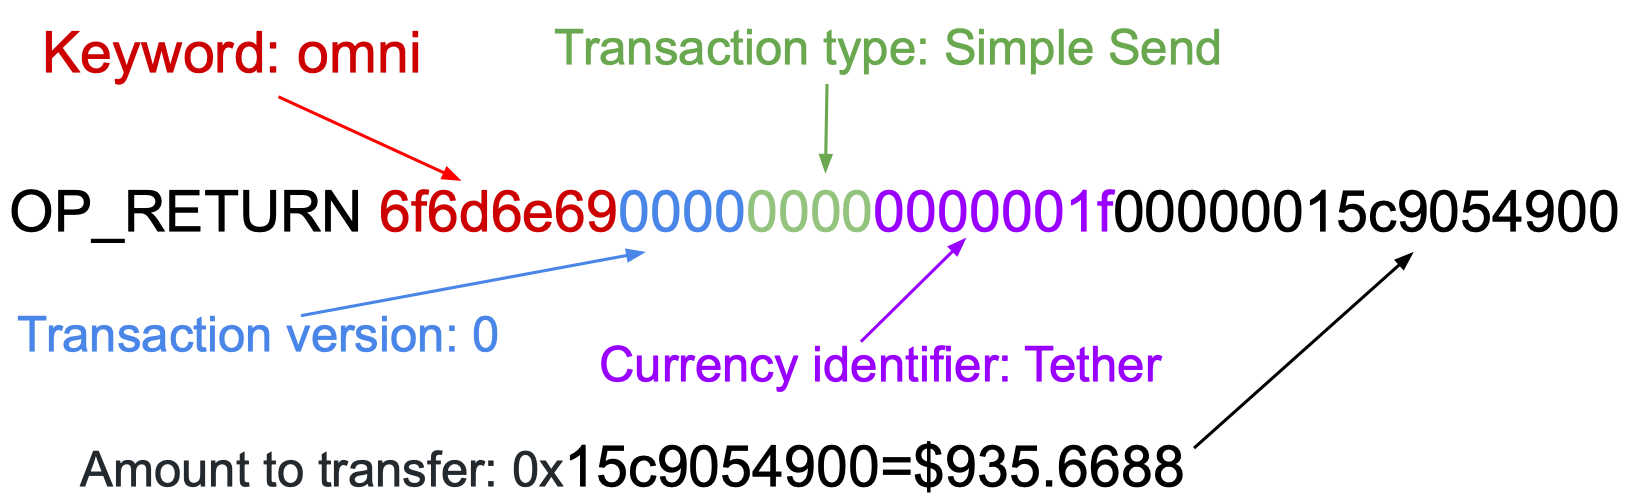
\includegraphics{figures/USDT}}%
	}
\caption{USDT}
\end{figure}


%[ref][https://www.blockchain.com/btc/tx/efc50d9e1f23e687e304cfca4ef2c5412b67d5737888ff80a0cbb6853cd865c]



\subsubsection*{OP\_GROUP}
The OP\_RETURN  scheme is more suitable to apply on mature blockchain, since it does not change the underlying blockchain protocol and will not risk forking. However, the weakness is that miners cannot verify its protocol, so there would be some security risks.

OP\_GROUP\cite{OP_GROUP}  is an improvement proposal of assets issuance on Bitcoin Cash (BCH)\cite{BCH} from Bitcoin Unlimited (BU). Thus, OP\_GROUP  supports transfer, destroy and insurance of Token. Since OP\_GROUP is an extension to the BCH script system,  it is part of the BCH protocol. Thus miners can do the verification, which is more reliable.

The basic “colored” pay 2 public key hash script would be like:

\lstset{basicstyle=\tiny,style=myListStyle}
\begin{lstlisting}[numbers=none]
OP_DATA(group address)
OP_GROUP
OP_DROP
OP_DUP
OP_HASH160
OP_DATA(pubkeyhash)
OP_EQUALVERIFY
OP_CHECKSIG
\end{lstlisting}

The main difference is simple, just adding a group address to distinguish different groups, and other operations, such as create and destroy assets, are similar.

% [ref]https://medium.com/@g.andrew.stone/bitcoin-scripting-applications-representative-tokens-ece42de81285

\subsection{OP\_TOKEN Design}

\subsubsection{Overview}

There is a unique token named LICENSE in OP\_TOKEN. The relevant regulatory entities, industry practitioners with public credibility within the ecosystem are invited to receive the licenses to oversight the compliances issues that might occur along the course of mainstream adoption of the protocol. Any entity planning to issue a token needs to be warranted with a license. Peers can transfer licenses as they are also tokens in nature. The originator must be extra careful in event of transferring in order to avoid non-compliance risk of transferring to a wrong person since the records is public and immutable.  
 

\subsubsection{License Creation}

Licenses are all generated in the genesis block and distributed to C preserved committee members. One smallest unit (QIT) can represent a license, one block has M coins, one coin= N QIT, so we have M*N license in total, which is sufficient for asset issuance.


\begin{lstlisting}[language=yaml, numbers=none,basicstyle=\footnotesize]
# C = 100, M = 10, N = 10^8 (M*N = 10 billion),
# all examples are based on this setting
# Ex1: Distribute licenses to the committee,
# M*N/C = 100 million for each member.
---
INPUTS:
	INPUT:
		PREVIOUS_OUTPUT: # (COINBASE of GENESIS)
			S: "DUP HASH160 [GEN] EQUALVERIFY CHECKSIG"
			V: 10000000000
		S: "[SIG] [GEN_PK]"
OUTPUTS:
	OUTPUT:
		S: "[LIC] TOKEN DROP DUP HASH160 [COMM1] EQUALVERIFY CHECKSIG"
		V: 100000000
	# ... ... (COMMITTEE MEMBER 2~99)
	OUTPUT:
		S: "[LIC] TOKEN DROP DUP HASH160 [COMM100] EQUALVERIFY CHECKSIG"
		V:100000000
	OUTPUT:
		S: "RETURN [DATA]"
		V: 0
\end{lstlisting}



\subsubsection{Issue a License}

The relevant entities must be warranted a license to issue assets. The entity can request a license from any committee member (C.M.). Once the license is granted and approved. These entities will receive a particular token from the C.M. and the Token is the licensed.

\lstset{basicstyle=\tiny,style=myListStyle}
\begin{lstlisting}[language=yaml, numbers=none,basicstyle=\footnotesize]
# Ex2: C.M. warrant a license to the issuer (ISS),
# note the license change will go back to the C.M.
---
INPUTS:
	- INPUT:
			PREVIOUS_OUTPUT:
				S: "[LIC] TOKEN DROP DUP HASH160 [COMM] EQUALVERIFY CHECKSIG"
				V: 100000000
			S: "[SIG] [COMM_PK]"
OUTPUTS:
	- OUTPUT:
			S: "[LIC] TOKEN DROP DUP HASH160 [ISS] EQUALVERIFY CHECKSIG"
			V: 1
	- OUTPUT: # License change
			S: "[LIC] TOKEN DROP DUP HASH160 [COMM] EQUALVERIFY CHECKSIG"
			V: 99999999
	- OUTPUT:
			S: "RETURN [DATA]"
			V: 0
\end{lstlisting}

\subsubsection{Issuance of assets}
Once the license is warranted, entities can issue assets; however, they cannot set the token amount arbitrarily. Instead, to issue a certain amount of assets requires converting the same amount of QITs. The Qitmeer network calls this process as "token mint". Just like the case in reality, to mint a gold coin requires the same weight of gold qits, tokens need the same amount of QITs.

The first advantage of issuance system is to guarantee tokens’ elementary intrinsic value; thus, it would significantly mitigate the price fluctuation. Another advantage is that tokens and native currency are no longer isolated islands of value, which are running in the same ecosystem and would improve the liquidity and make the whole network stable.

\lstset{basicstyle=\tiny,style=myListStyle}
\begin{lstlisting}[language=yaml, numbers=none,basicstyle=\footnotesize]
# Ex3: Convert 100000000 QIT, i.e. 1 MEER,
# to 100000000 units of the new token,
# note the license will go back to the issuer for future issuance.
INPUTS:
	- INPUT:
			PREVIOUS_OUTPUT: #(1 LICENSE)
				S: "[LIC] TOKEN DROP DUP HASH160 [ISS] EQUALVERIFY CHECKSIG"
				V: 1
			S: "[SIG] [LIC_PK]"
	- INPUT:
			PREVIOUS_OUTPUT: #(1 Qitmeer Coin)
				S "DUP HASH160 [COIN] EQUALVERIFY CHECKSIG"
				V: 100000000
			S: "[SIG] [COIN_PK]"
OUTPUTS:
	- OUTPUT: # License returns to the issuer
			S: "[LIC] TOKEN DROP DUP HASH160 [ISS] EQUALVERIFY CHECKSIG"
			V: 1
	- OUTPUT:
			S: "[TOK] TOKEN DROP DUP HASH160 [PK] EQUALVERIFY CHECKSIG"
			V: 100000000
	- OUTPUT:
			S: "RETURN [DATA]"
			V: 0
\end{lstlisting}

\subsubsection{Transfer of the Assets}

The entities can transfer assets to each other. Moreover, the entity could transfer multiple assets within one transaction. The transaction needs to ensure the input sum of each asset equals the output sum of each asset.

\lstset{basicstyle=\tiny,style=myListStyle}
\begin{lstlisting}[language=yaml, numbers=none,basicstyle=\footnotesize]
# Ex4: Alice exchanges her 100 RMB token with Bob's 20 USD token.
INPUTS:
	- INPUT:
			PREVIOUS_OUTPUT:
				S: "[RMB] TOKEN DROP DUP HASH160 [A_PKH] EQUALVERIFY CHECKSIG"
				V: 100
			S: "[A_SIG] 0X83 [A_PK]"
	- INPUT:
			PREVIOUS_OUTPUT:
				S: "[USD] TOKEN DROP DUP HASH160 [B_PKH] EQUALVERIFY CHECKSIG"
				V: 20
			S: "[B_SIG] 0X83 [B_PK]"
OUTPUTS:
	- OUTPUT:
			S: "[USD] TOKEN DROP DUP HASH160 [A_PKH] CHECKSIG"
			V: 20
	- OUTPUT:
			S: "[RMB] TOKEN DROP DUP HASH160 [B_PKH] CHECKIG"
			V: 100
\end{lstlisting}


\subsubsection{Token Melt}

Token Melt is the reversed process of Token Mint, i.e., conversion from tokens to native currency. The total amount of qit is constant, either in the form of Native QIT or Token QIT. However, it is allowed to transform a token and convert native currency. Issuers can melt their coins to reduce liquidity in order to keep the price stable, which is practical to implement stable coins. Token Melt guarantees the tokens fundamental value, just like the minimum value of a gold coin is the same weight of gold.   


Melt guarantees the tokens fundamental value, just like the minimum value of a gold coin is the same weight of gold.

\lstset{basicstyle=\tiny,style=myListStyle}
\begin{lstlisting}[language=yaml, numbers=none,basicstyle=\footnotesize]
# Ex5: Melt 100 token qits into 100 native qits
INPUTS:
	- INPUT:
			PREVIOUS_OUTPUT:
				S: "[TOK] TOKEN DROP DUP HASH160 [ISS] EQUALVERIFY CHECKSIG"
				V: 100
			S: "[SIG] [ISS_PK]"
OUTPUTS:
	- OUTPUT:
			S: "DUP HASH160 [COIN] EQUALVERIFY CHECKSIG"
			V: 100
	- OUTPUT:
			S: "RETURN [DATA]"
		V: 0
\end{lstlisting}


\section{Consensus Protocol}

BlockDAG is a high throughput framework with highlights in fully decentralized and high security. Futhermore, it is a natural extension to classical bitcoin paradigm, meaning it would inherit most  long time verified qualities of bitcoin and is expected stronger stability.

Qitmeer introduces GHOSTDAG as fundamental protocol to achieve high throughput linearly ordering service, with fast confirmation guaranteed by SPECTRE protocol.

\subsection{From BlockChain To BlockDAG}
Bitcoin does not scale due to protocol restrain. According to Nakamoto Consensus, i.e., longest-chain rule, 1 MB block size and 10 minutes block rate confine bitcoin to reach only 7 TPS theoretical throughput, regardless how great the bandwidth and how fast propagation delay is.

The most intuitive way to increase scalability is to shorten block time or enlarge block size. The reason why Nakamoto Satoshi did not adopt is because that will bring forks, as well as distracting the hash power from the main chain, thus causing security vulnerability.

GHOST protocol introduces heaviest-tree consensus to keep the forks without sacrificing security. Note that here BlockChain has transformed into a BlockTree. Since the largest subtree has concentrated the majority hash power, the security is as high as bitcoin. The main chain is the chain of blocks from the genesis to  a leaf with the greatest number of descendants, other blocks are off-chain blocks. Only main chain blocks contribute throughput, off-chain blocks help

BlockTree has dramatically increased throughput because of the higher Block Creation Rate or greater Block Size. However, there is still a waste of the transactions in off-chain blocks which should contribute to the throughput as well. Inclusive\cite{Inclusive} protocol proposes a new data structure of ledger, where every block confirms every unconfirmed block. This improvement upgrades a BlockTree to a BlockDAG.

Through the development history from BlockChain to BlockDAG, it may indicate  that BlockChain is a particular case of BlockDAG in the event of low throughput, which means both are the same in essence. As a result,  it is the scalability solution whose paradigm is the closest to the bitcoin network. BlockDAG is robust since it inherits all the long-time-proved stable features of bitcoin,  as well as it could scale infinitely at the protocol level, only limited physically, such as, bandwidth or propagation delay. A robust public chain is the optimal basis for incorporating further scaling solutions, such as sharding and state-channels, thus BlockDAG is the preferred scaling solution of Qitmeer.


\begin{figure}[hbt]
	\centerline{%
	   \resizebox{0.8\textwidth}{!}{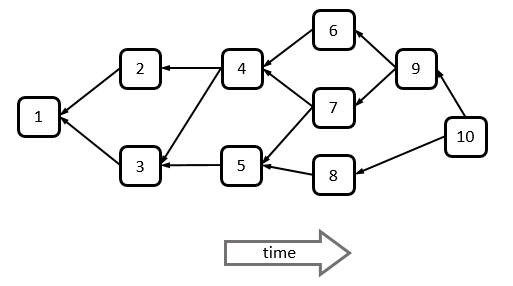
\includegraphics{figures/DAG.png}}%
	}
\caption{DAG}
\end{figure}

\subsection{GHOSTDAG}
GhostDAG, formerly Phantom, is the first BlockDAG protocol supporting block total ordering. Compared to SPECTRE, it guarantees Strong Liveness that all the blocks , including dishonest blocks, will get confirmed in a definite time, making consensus protocol more robust.

\subsubsection{Intuition}

Here is the idea behind GHOSTDAG. Suppose that the maximal limits of network propagation delay and block creation
rate are constant. It is intuitive that if nodes behave honestly, it forms a subgraph where each block has at most a constant number of forks. We denote
this constant number as $k$. $k$ can be calculated from propagation time and
block creation rate. The subgraph is denoted as a $k$-cluster. The biggest
$k$-cluster is called a blue set. Those blocks outside the blue set are called
red set.

If we can traverse from block $x$ to block $y$ by following the parent
references within each block, then we say that there's a partial order between
$x$ and $y$, and $y$ is prior to $x$. For example in the following figure, we
can traverse from block J to A through B, so there's a partial order between A
and J, and A is prior to J. Note not all blocks have partial orders with other
blocks. For example, there are no partial orders between B, C and D.  The block set where no partial order exists is an anticone. The size of any anticone in
a $k$-cluster is at most $k$.

\begin{figure}[ht]
	\centerline{%
	   \resizebox{0.8\textwidth}{!}{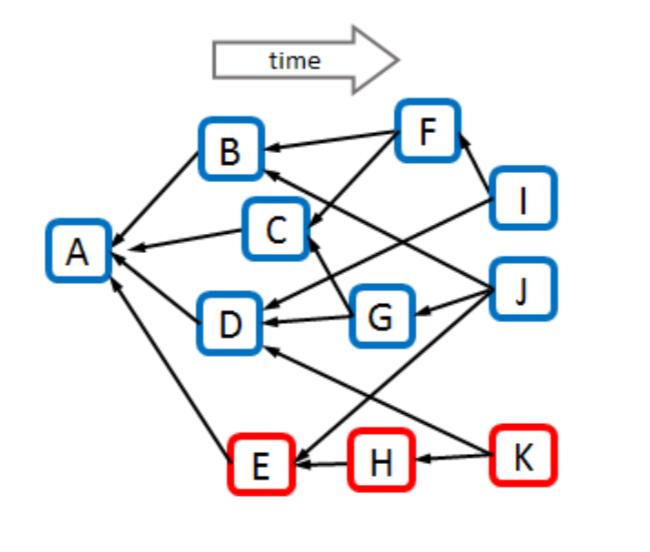
\includegraphics{figures/GHOSTDAG}}%
	}
\caption{GHOSTDAG}
\end{figure}


\subsubsection{Ordering}

GHOSTDAG orders the DAG ledger in a way that favours blue blocks and penalizes
red ones. So, if two blocks X and Y have no partial order from the graph, the one in blue set is prior to the one in the red set.

The coloring algorithm is based on a block's past set, also known as ancestors, since the past set gets fixed after a block generated, the blue set will get fixed as well. Therefore, each block could choose the parent with maximal blue set as its main parent. Then, repeat the process of finding main parent from the tip blocks extending to the genesis block, finally we could figure out a unique block chain that is under agreement by the majority of the network, we name this block chain as main chain. Once main chain is identified, all the blocks could form a linearly order by reference to it. 


\begin{figure}[ht]
	\centerline{%
	   \resizebox{0.8\textwidth}{!}{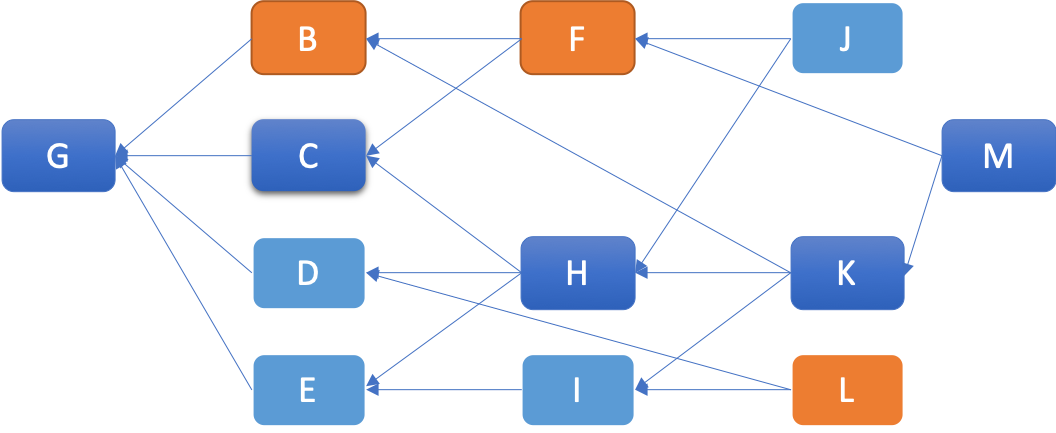
\includegraphics{figures/Ordering}}%
	}
\caption{GhostDAG Ordering}
\end{figure}

For example in figure 5, this is a 3-cluster DAG. 

\begin{enumerate}
	\item Add genesis block G in blue set
	\item Add B,C,D,E to blue set, since none of them has an anticone greater than 3
	\item Since the blue set of H is greater than that of F and I, so add H in blue set. Add I to blue set because its anticone size is only 2; Add mark B and F in red set for anticone size greater than 3
	\item turn for J,K,L . Both past set size and blue set size of J and K are the same, so currently there are two possible main chain, G-C-H-J and G-C-H-K 
	\item since M's blue set is greater than that of J and L, M is added to blue set, so there is only one main chain left, G-C-H-K-M. Add J to blue set due to small anticone size then add F, L to red set due to big anticone size, now red set and blue set as well as main chain are identified
	\item the order is G-C-D-E-H-I-B-K-F-j-M-L
\end{enumerate}

\subsection{SPECTRE}
SPECTRE\cite{SPECTRE} is a BlockDAG based consensus protocol that achieves fast confirmation and high throughput with 50\% attack resilience. SPECTRE has weak liveness, it guarantees fast confirmations only for honest users rather than all users.

There is a trade-off between liveness and fast confirmation, whereby SPECTRE prioritizes the latter due to weak liveness only affects malicious users, that enables SPECTRE to be a suitable protocol for payment network. In the event malicious users launch double spending attack, their transactions are likely to be delayed indefinitely.

SPECTRE is a stateless transaction model, whereby there is no need to gain a total ordering over all the blocks. Only when two blocks conflicting that a pairwise ordering is needed. SPECTRE employs a voting algorithm to decide which block wins when two blocks
conflict. Suppose block $x$ has a conflicting transaction with another
transaction in block $y$, and also suppose that block $z$ is voting on them with
the following rules:

\begin{enumerate}
	\item If $z$ is in $x$'s future but not in $y$'s future, $z$ votes for
		$x$ in favor of $y$, denoted as $x \prec y$, and vice versa.
	\item If both $x$ and $y$ are in the past of $z$, then $z$ follows the majority votes in its past.
	\item If neither $x$ nor $y$ is in the past of $z$, then $z$ follows the majority votes in its future.
	\item Both $x$ and $y$ vote for themselves unless one is in the past of
		the other.
\end{enumerate}


Here's an example of how a new block (number 12 in the figure below) votes:

\begin{figure}[ht]
	\centerline{%
	   \resizebox{0.8\textwidth}{!}{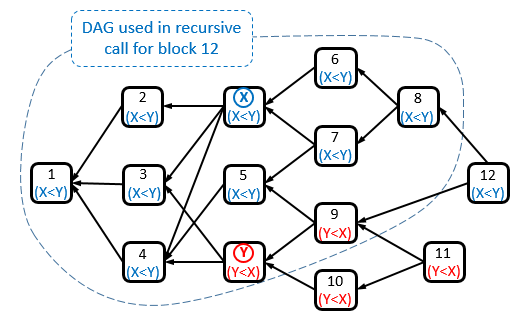
\includegraphics{figures/SPECTRE}}%
	}
\caption{An example of the voting procedure in the DAG for blocks $x$ and $y$ in SPECTRE}
\end{figure}

According to rule 4, block $x$ votes for $x \prec y$, block $y$ votes for $y
\prec x$.

According to rule 1, blocks 6, 7 and 8 vote for $x \prec y$, blocks 9, 10 and 11
vote for $y \prec x$.

According to rule 2, block 12 votes according to its past. Since not all blocks
of its past have voted, we change global view to block 12's local view, which
means block 10 and 11 are excluded.

According to rule 3, block 5 votes for $x \prec y$, since the majority of its
future vote in favor of $x$ over $y$ (blocks 7, 8 versus block 9). Note that the
current view is block 12's local view and block 11 is excluded, so we cannot
take its vote.

Also according to rule 3, blocks 1\textasciitilde4 vote for $x \prec y$.

Now all the blocks in block 12's past have voted. Block $x$ gets 10 votes. Block
$y$ gets 2 votes. Block 12 follows the majority and votes for $x \prec y$ thus.


\subsubsection*{Confirmation Time}

When a node $v$ receives a block $x$, it loops to calculate the  risk of
the block. It accepts the block when the risk is smaller than a given threshold
$\epsilon$. The confirmation time of block $x$ in node $v$ is the time
since $x$ is received by $v$ until $x$ is accepted by $v$.

The following algorithm below calculates the  risk of block $x$ in
$G_t^v$, where $G_t^v$ is the block DAG that $v$ observes at time $t$.

\begin{codebox}
\Procname{\proc{Risk}$(G_t^v, x)$}
\li \If $time\_now < publication(x)$
\li   \Then
        \Return 1
      \End
\li $T \gets time\_now - received^v(x)$
\li $G_x \gets G_{received^v(x) + 2 \cdot d} \cup future(x, G_t^v)$
\li $g \gets \min_{x' \in \overline{ainticone}(x,G_x)} |future(x',G_x)|$
\li \Return $risk\_hidden(T,g)$
\end{codebox}

The formula $risk\_hidden(T,g)$ is defined as:

$$
risk\_hidden(T,g) := \sum_{l=0}^{\infty} \pi(l) \sum_{m=0}^{\infty} Poiss((T + 2
\cdot d) \cdot \alpha \cdot \lambda, m) \cdot \left(\frac{\alpha}{1 -
\alpha}\right)^{(g - l - m)^+},
$$

where

\begin{itemize}
	\item $d$ is the upper bound on the recent delay diameter in the network,
	\item $\alpha$ is the attacker’s relative computational power,
	\item $\lambda$ is the block creation rate,
	\item $Poiss(a, b)$ is defined as $e^{-a} \cdot \frac{a^b}{b!}$,
	\item $x^+$ is defined as $\max\{0, x\}$,
	\item and $\pi$ is the stationary distribution which we will explain below.
\end{itemize}

$risk\_hidden(T,g)$ upper bounds the probability that block $x$ is preceded by
some attacker’s block $y$ in pairwise order, where $y$ is published later than
$x$.

$\pi$ is actually a vector. Informally, it is the statistical distribution of
how much more blocks attacker nodes have created than honest nodes have created
since block $x$ is published, which is called gap in the SPECTRE paper. $\pi(l)$
is the probability that the value of gap is $l$.

The value of gap changes as time goes on, forming a random walk which induces an
ergodic Markov chain. Theoretically, it could be any integer ranging from
negative infinity to positive infinity. In the worst case, it is always
non-negative. Only when the gap is non-negative is there a risk for block $x$ to
be received less or equal votes than some attacker’s block $y$ which is
published later than $x$, so that $y$ precedes $x$ in pairwise order. This is
why in the formula of $risk\_hidden$ the index $l$, i.e. the value of gap,
starts out equal to 0 instead of negative infinity.

Since the random walk of $l$ induces an ergodic Markov chain, $l$ has a unique
stationary distribution, which is $\pi$. In order to calculate $\pi$, we need to
calculate the transition probability matrix of the random walk.

Suppose that the value of $l$ ranges from 0 to $N$, where $N$ is infinity in the
above definition. We define the transition probability matrix as an $N$ by $N$
matrix $T$. We also denote by $\delta := \alpha \cdot \lambda \cdot d$. For all
$1 \leq l < N - 1$, $T_{l-1,l} = 1 - \alpha, T_{l+1,l} = \alpha$, and for $l = N
- 1$: $T_{l-1,l} = 1 - \alpha, T_{l,l} = \alpha$. The first column of the matrix
is defined by: $T_{0,0} := (1 - \alpha) \cdot e^{-\delta}, T_{1,0} = e^{-\delta}
\cdot \alpha + e^{-\delta} \cdot \delta$, for $1 < l < N - 1$: $T_{l,0} =
e^{-\delta} \cdot \frac{\delta^l}{l!}$, and $T_{N-1,0} = 1 - e^{-\delta} \cdot
\left[\frac{\delta^0}{0!} + \frac{\delta^1}{1!} + \cdots +
\frac{\delta^{N-2}}{(N-2)!}\right]$.  $\pi$ is the eigenvector of $T$
corresponding to the eigenvalue 1, where $\pi(l) \geq 0$ and the sum of $\pi$ is
1.

In practice, $\pi(l)$ is very close to zero when $l$ is very large, so we can
just pick some $N \gg 1$ instead of infinity. Therefore, the formula of
$risk\_hidden$ becomes

$$
risk\_hidden(T,g) = \sum_{l=0}^{N} \pi(l) \sum_{m=0}^{\infty} Poiss((T + 2 \cdot
d) \cdot \alpha \cdot \lambda, m) \cdot \left(\frac{\alpha}{1-\alpha}\right)^{(g
- l - m)^+}.
$$

It is recommended to calculate $\pi$ with some well-tested Markov chain library such
as the markovchain package in R.

The sum of series with index $m$ seems to be a sum of infinite series. However,
for $m > g - l$ we have $(g - l - m)^+ = 0$ and
$\left(\frac{\alpha}{1-\alpha}\right)^{(g - l - m)^+} = 1$.

Therefore, the formula of $risk\_hidden$ can be further converted as below,
where $Poiss_{cdf}$ is the cumulative distribution function (CDF) of Poisson
distribution.

\begin{align*}
risk\_hidden(T,g)
=& \sum_{l=0}^{N}\pi(l)\sum_{m=0}^{\infty}Poiss((T+2 \cdot d) \cdot \alpha \cdot \lambda, m) \cdot (\frac{\alpha}{1-\alpha})^{(g-l-m)^+} \\
=& \sum_{l=0}^{N}\pi(l) (\sum_{m=0}^{g-l}Poiss((T+2 \cdot d) \cdot \alpha
	\cdot \lambda, m) \cdot (\frac{\alpha}{1-\alpha})^{(g-l-m)} + \\
& \sum_{m=(g-l+1)^+}^{\infty}Poiss((T+2 \cdot d) \cdot \alpha \cdot \lambda, m)) \\
=& \sum_{l=0}^{N}\pi(l) ( \sum_{m=0}^{g-l}Poiss((T+2 \cdot d) \cdot
	\alpha \cdot \lambda, m) \cdot (\frac{\alpha}{1-\alpha})^{(g-l-m)} + \\
& (1 - Poiss_{cdf} ((T+2 \cdot d) \cdot \alpha \cdot \lambda, (g-l)^+))).
\end{align*}

With the converted formula we are able to calculate $risk\_hidden$ in numerical way. Figure 5 simulates the confirmation time on different block rates, it show that SPECTRE could achieve 5 seconds confirmation time on block rates higher than 10 blocks per second and 10\% faulty percentage, which is considerably promising.

\begin{figure}[ht]
	\centerline{%
	   \resizebox{0.8\textwidth}{!}{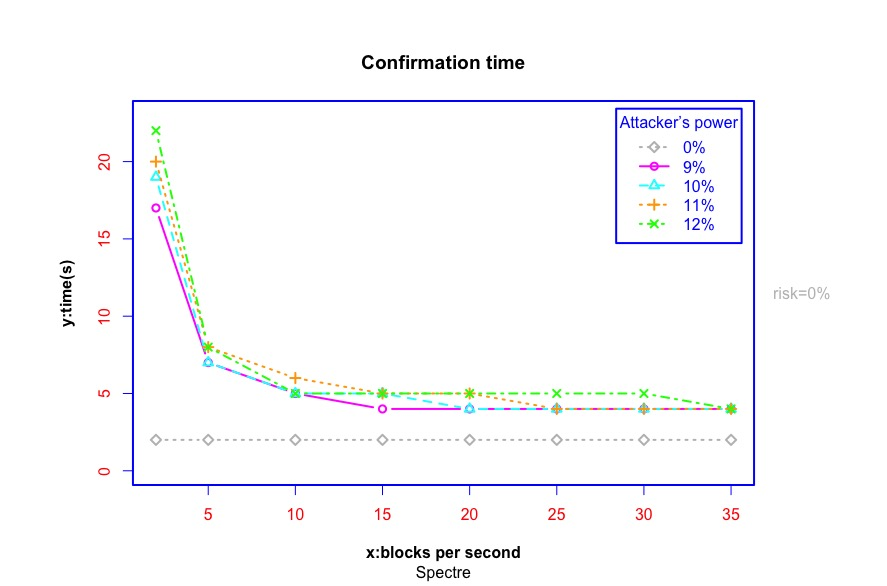
\includegraphics{figures/confirmation.jpeg}}%
	}
\caption{Confirmation Time}
\end{figure}


\subsection{Mining Algorithm}
BlockDAG’s collaboration model provides much more fairness than the competition model of BlockChain on the protocol perspective. Every node gets rewards according to its contribution, regardless of how much hash power it possess. Qitmeer favors fairness over the scalability owing to the former is more in line with true spirit of blockchain. The intention of Nakamoto Consensus is fair - every node votes with electricity; however, only a small bunch of the mining pools have the odds to participate in consensus. solo miners suffer huge risk since they have to wait for an uncertain time, quite long in most cases, to mine a block to cover their cost; thus finally it will have to turn to the mining pools. BlockDAG includes every miner’s block, the miners have a stable expectation on their rewards ,  therefore it is not too necessary for them to join a mining pool.


In addition, the mining algorithm is  another factor of fairness. Mining fairness refers to a certain amount of mining cost, such as electricity in POW, should derive the relatively equivalent amount of hash power. Practically, the ASIC mining rigs have much more mining efficiency than their prices.

\subsubsection{Cuckoo-Cycle-PoW}
Proof-of-Work(PoW) is used to confirm transactions and produces new blocks, and acts as the driving force in PoW based cryptocurrencies. PoW must not enable a participant to have a significant advantage over another participant. That is what Satoshi proposed: "Proof-of-work is essentially one-CPU-one-vote."

However, most widely used proof-of-work algorithms, such as SHA-256, Blake2b, Scrypt, are more efficient on ASIC devices when compared to CPUs and GPUs. This can lead to ASIC owners posses a much larger voting power than CPU and GPU owners, which violates the “one-CPU-one-vote” principle.

Cuckoo-Cycle-PoW, a graph-theoretic proof-of-work ASIC-Resistant mining algorithm, it is designed to find certain subgraphs in large pseudo-random graphs. In particular, Search for cycles of specified length L in a bipartite graph with M edges of N nodes. If a cycle is found and the hash difficulty is less than the target difficulty, the cuckoo cycle PoW is completed.

\textbf{Edge(Node) generation}

For the sake of simplicity, we define 32 edges for the bipartite graph. We call the SIPHASH function twice to create two edge endpoints(U and V), with the first input value being 2 * nonce, and the second 2 * nonce+1. The key for this function is based on a hash of a block header.

\begin{equation}
{U = SIPHASH(headerHash, 2*nonce) \mod 31}
\end{equation}
\begin{equation}
{V = SIPHASH(headerHash, 2*nonce+1) \mod 31}
\end{equation}

where,
\begin{equation}
0\leq\ {\bf nonce} \leq 31
\end{equation}it is any number between 0 and 31. Each nonce corresponds to two edge endpoints(U and V).

To throw 32 edges into a graph, randomly:

\begin{figure}[ht]
	\centerline{%
		 \resizebox{0.8\textwidth}{!}{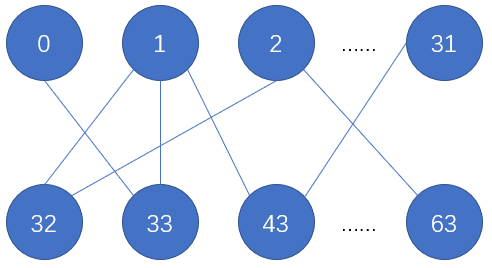
\includegraphics{figures/edge_generation}}%
	}
	\caption{Building Nodes.}
\end{figure}


\textbf{Edge Trimming}

There is a special edge in bipartite graph, which is leaf edge, and could never be part of a cycle. Leaf edge has a feature that the nodes it connects must have at least one node with the degree of the nodes being one. By eliminating leaf edge in the bipartite graph, it could greatly reduce the complexity of the graph, thus speeding up finding cycle from the bipartite graph.

\begin{figure}[ht]
	\centerline{%
		 \resizebox{0.8\textwidth}{!}{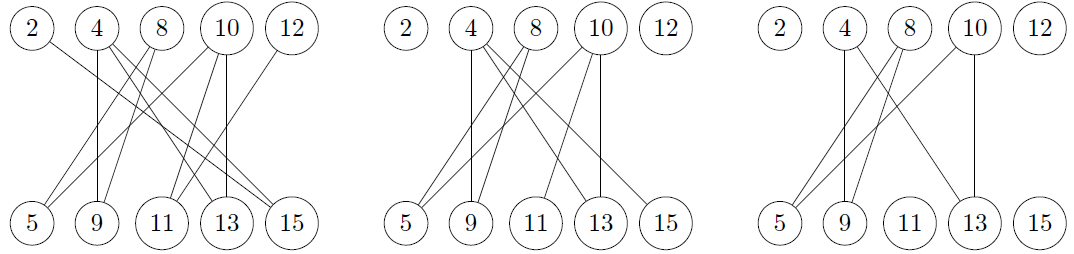
\includegraphics{figures/edge_trimming}}%
	}
	\caption{Trimming of edges which cannot be part of a cycle.}
\end{figure}

\begin{itemize}
	\item Step 1: node 0, node 3 and node 10 are one degree nodes, eliminating the edge (0,13), (6, 3) and the edge (10,9).
	\item Step 2: node 9 and node 13 are one degree nodes, eliminating the edge (8,9) and the edge (2,13).
	\item Step 3: node 8 is one degree nodes, eliminating the edge (8,11).
\end{itemize}


\textbf{Cycle detection}

After edge trimming, if a cycle of length L is found, we think we have found a solution to this problem.
we store the cycle edges in a set and put the nonce of the generated cycle in a set and
return as the result of cycle detection.


\textbf{Difficulty control}

The difficulty of finding a cycle in the graph is proportional to M/N. Here M stands for edges of the graph.
N stands for nodes of the graph. However, the difficulty of finding a cycle in the graph change is not smooth.
For crypto currencies, difficulty control must be scale in precisely controlled manner. The usual practice is
that the ratio of M/N remain fixed, such as M/N = 1/2.

Thus in the actual use, it also adds a hash difficulty control similar to Bitcoin. The digest of the cycle nonces is obtained by a hash function,
and then compared with the target difficulty.

\subsubsection{Difficulty Adjustment}
To keep block creation rate stable, Qitmeer adjust mining difficulty periodically. 
The adjustment rule is deviated from BlockChain due to forks of BlockDAG

\subsubsection*{Blue Set Based}
Rather than based on all the blocks, Qitmeer adjustment different merely on Blue blocks. 

\subsubsection*{Dynamic adjustment interval}
It is complicated to adjust the difficulty every fixed number of blue blocks, because different block has different blue set, leading difficult to make a agreement on which block to be the adjustment point.

Qitmeer exploits main chain to overcome this problem. The rule is:

\begin{enumerate}
	\item  Wait until 144 blocks newer than last adjustment point in main chain.
    \item  Calculate the actual time, which is the time span from last adjustment point to now.
    \item  Calculate number of new blue blocks created.
    \item  Calculate the expected time of those blue blocks by multiply the number with block time.
    \item  Adjust the difficulty by comparing expected time and actual time.
\end{enumerate}



\section{Incentive system}
The economic drive for the miners to work for a blockchain network is a reasonable incentive system. Qitmeer distributes rewards in a fully decentralized way - mining. Qitmeer concerns fairness among all the nodes, regardless how much power one owns. For miners with strong hash power, they may strive for the block reward, which is abundant, though more competition intensive ; for those with less power, they still got the chance to share transaction fee, first come first serve.

\subsection{Block Reward}
Miners create a block, including all the unconfirmed transactions, and add a transaction funding to themselves with a commonly admitted amount, then find the cryptic solution and broadcast it to the network. That's simply how mining works, and  this self transfer is called coinbase reward or block reward. 

Block reward is considerable and incentives miners to compete intensively to obtain.  BlockDAG paradigm is a collaboration model, therefore the threshold could be lower and the distribution  fairer, however, block reward is essentially a scare resource that requires miners with considerable hash power to take part in this game.

\subsection*{Blue Set Only}
As clarified in Consensus Protocol section, GhostDAG protocol colors the honest blocks with blue and the dishonest with red. Qitmeer gives block rewards only to those blocks colored as blue.
Qitmeer identifies merely block rewards of blue blocks as valid, the reasons as below.

\subsubsection*{Encourage miners working actively}
The network is rely on miners working hard to consolidate security. Competition in BlockDAG paradigm is not be as intensive as that in BlockChain, therefore we need to encourage miners working positively to better secure the network. Since working passively has higher probability to be identified as red block, miners will work hard to avoid such situation.

\subsubsection*{Resilient to potential attack}
The instinct of BlockDAG to incorporate forks makes it more inclusive than BlockChain. However, it would reduce the cost to perform an attack because even the failing blocks will be included in the ledger. Since the failing blocks are probably identified as red blocks and paid nothing, it increases the investment of attack dramatically and attacker would not carry on attacks abruptly.

\subsection{Transaction Fee}
Blue Set policy would consolidate the security considerably, nonetheless it brings discrimination to those miners with less hash power or worse network traffic condition. Perhaps they are honest miners as well but still are identified as "dishonest" due to consensus protocol's limitation. Therefore, we could utilize transaction fee to compensate those less powerful honest miners. 

\subsubsection{Every block gets paid transaction fee}
The block reward aims at security while the transaction fee is targeting more on underlying service - value transfer. So the reward policy for transaction fee cares more about fairness, if you devoted to the network, the network would pay you accordingly regardless how much hash power you have.

Other than block reward is orientated merely from  blue blocks, transaction fee is transferred on every blocks, even marked as red. So, miners get paid as long as they work hard. E.g., due to locality, the miners prioritizes to incorporate transactions geographically around them. So, even if their blocks broadcast slower due to poor network traffic and eventually marked as red, they still could receive those transaction fee.

\subsubsection{Weighted transaction fee}
Due to asynchronous block submission, BlockDAG protocols inevitably incorporate repeating transactions, called transaction collisions.
Miners tend to pack the transaction with higher fees to maximize their profit. This will result in high repetition rates of blocks. Repeated transactions will not contribute to the throughput, what is more, low fee transactions would wait indefinite time to get confirmed. In a fully decentralized network, nodes cannot coordinate each other to avoid collision, leaving the only option to devise a sophisticated incentive mechanism to penalize the selfish mining behaviors.

The intuitive way to solve this challenge is to share the transaction fee, and this method will make all the miners reach a Nash equilibrium that all the miners will choose transactions randomly from their memory pools. This approach will considerably reduce transactions collision; however, users would no longer pay higher fees to boost their transaction confirmation, so this policy would break the functionality of transaction fee.

Inspired by inclusive protocol, Qitmeer takes on a simpler Weighted Transaction Fee policy to balance the functionality and collision. The policy is really simple, higher transaction has accordingly higher probability to be included. E.g., if one transaction fee is 2 times higher than another, it is two times more likely to be picked from the mempool.

\subsubsection{First Come First Serve}
Inspired by Inclusive protocol as well, Qitmeer takes on First Come First Serve policy for transaction fee. The idea is straightforward, whoever is the first one to include the transaction wins the transaction fee.

However, the implementation of this idea is not as easy as expected and is not covered in Inclusive paper. By bitcoin's diagram, miners collect transactions fee in coinbase as well, at this phrase, its order is undetermined. Simply put, the miner has no idea which transaction will be the first included than the rest of the network, the only way is to assume all the the transactions will be the first and collect all the fee, but actually some of them would be identified invalid.

Qitmeer's solution to this problem is to balance this coinbase transaction when the miners tried to spend it. For instance, if a miner creates a block with 3 transactions with 0.1 meer fee each, finally identified 2 out of 3 are first included, the rest is not. When the miner creates a transaction to spend this block reward, he has to add an output pointing to a special address with amount 0.1 to burn the redundant fee.

\section{Protocols and Interoperability}
BlockChain is the digital infrastructure for decentralized financial system, which would evolve into a complete ecosystem in the course of reaching maturity. This session analyses the typical applications available on  Qitmeer network and the protocols for interaction with Qitmeer. 

\subsection{Mining Protocol}
\subsubsection{Proof-of-work Algorithm}

The mining protocol is resistant to the centralization of mining power, which enables miner utilize almost all parts of commodity hardware (GPUs, CPUs).
Therefore, Qitmeer uses a Proof-Of-Work algorithm called Cuckoo Cycle\cite{cuckoocycle},
a memory-hard algorithm. This algorithm is designed to find certain subgraphs in large pseudo-random graphs.
An introduction of Qitmeer proof-of-work can be found here.\cite{qitmeerpow}

\subsubsection{Mining Protocol}

\begin{figure}[ht]
	\centerline{%
		\resizebox{0.8\textwidth}{!}{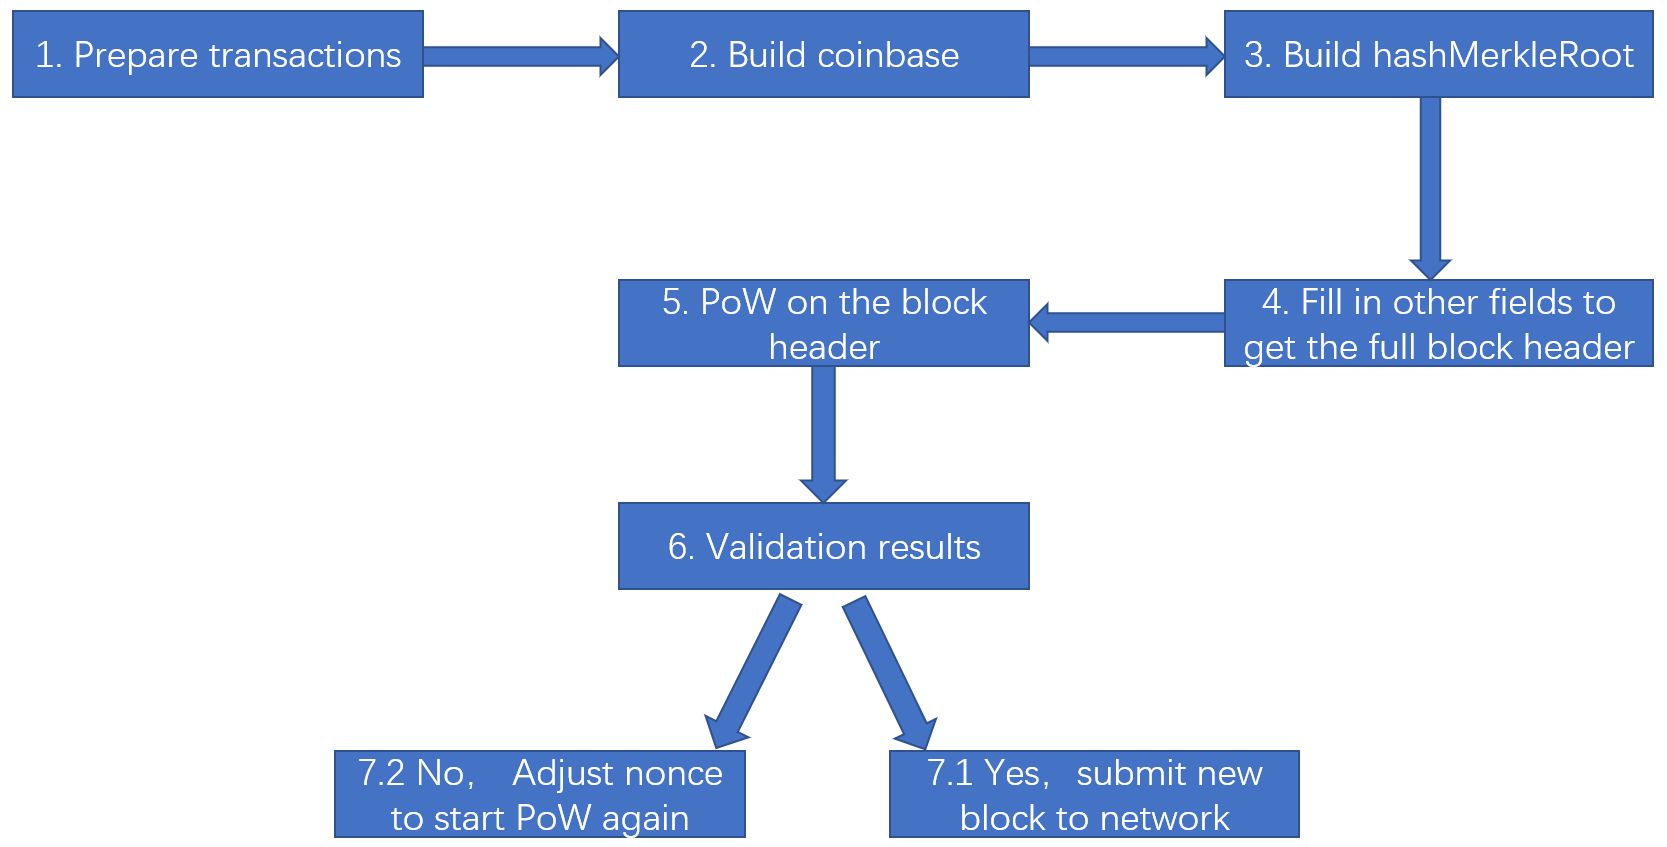
\includegraphics{figures/mining_process}}%
	}
	\caption{Mining process.}
\end{figure}

Qitmeer supports getblocktemplate mining protocol. It make the miner to decide which transactions are put in the block. The miner send a request to the Qitmeer full node by getblocktemplate RPC.
\begin{lstlisting}
{
	"jsonrpc": "2.0",
	"method": "getBlockTemplate",
	"params": [
				[
					"'$capabilities'"
				]
			],
	"id": 1
}
\end{lstlisting}
getblocktemplate return a JSON Object.
\begin{lstlisting}
{
	"jsonrpc": "2.0",
	"id": 1,
	"result": {
		"bits": "207fffff",
		"stateroot": "0000000000000000000000000000000000000000000000000000000000000000",
		"curtime": 1567323822,
		"height": 6,
		"previousblockhash": "50474e0a6f88f2f1aee7a0134a7be4b6e5ab6a7c9ba440b6c11c54494ca89d32",
		"sigoplimit": 80000,
		"sizelimit": 1310720,
		"weightlimit": 4000000,
		"parents": [
		{
		"data": "329da84c49541cc1b640a49b7c6aabe5b6e47b4a13a0e7aef1f2886f0a4e4750",
		"hash": "50474e0a6f88f2f1aee7a0134a7be4b6e5ab6a7c9ba440b6c11c54494ca89d32"
		}
		],
		"transactions": [],
		"version": 4,
		"coinbaseaux": {
		"flags": "092f7169746d6565722f"
		},
		"coinbasevalue": 45000000000,
		"longpollid": "50474e0a6f88f2f1aee7a0134a7be4b6e5ab6a7c9ba440b6c11c54494ca89d32-1567323822",
		"target": "7fffff0000000000000000000000000000000000000000000000000000000000",
		"maxtime": 1567331022,
		"mintime": 1567323743,
		"mutable": [
		"time",
		"transactions/add",
		"prevblock",
		"coinbase/append"
		],
		"noncerange": "00000000ffffffff",
		"capabilities": [
		"proposal"
		]
	}
}
\end{lstlisting}

Then the miner start PoW using the data from getblocktemplate RPC. If it get the right 'answer', submiting the potential block by submitblock RPC.
\begin{lstlisting}
{
	"jsonrpc": "2.0",
	"id": 1,
	"method": "submitBlock",
	"params": [
	"data"
	]
}
\end{lstlisting}

\subsubsection{Miner Capability}

The Qitmeer-Miner supports both solo mining and pool mining.

\subsubsection*{Solo}
If the miner  decided to mine Qitmeer without joining a pool, he would launch Solo mining mode. Solo miner connects one full node, call RPC service to mine blocks. Solo miner is recommended GPU implementation to gain better efficiency.

\subsubsection*{Pool}
Qitmeer mining pools support stratum mining protocol as most PoW mining pools do.
For example:

\emph{miner.exe -o stratum+tcp://serverIp:3177 -m YourWalletAddress.YourMachineId}

\subsection{Wallet Protocol}
\subsubsection{Overview}
   The blockchain wallet itself does not store any digital currency, and is primarily a computer program for creating digital currency transactions, tracking balances, and making it easy for users to manage addresses and private keys. Wallet software is the foundation of the whole block chain ecological development, any industry service can be realized through a block chain wallet value, block chain technology itself will reconstruct the traditional Internet business model in its own way. 
\subsection*{Openness}
   An excellent blockchain public chain project should be more inclusive and open. Therefore, in addition to its own official wallet, Qitmeer has designed all interfaces and SDK for third-party wallet development at the beginning of development. Third party wallet institutions can use these interfaces to develop a variety of wallet programs that support Qitmeer Token transactions. Including: HD wallet, SPV wallet, browser wallet to meet a variety of user needs.
\subsection*{How to create a wallet}
   The following is a simple wallet creation and transaction steps:
\begin{enumerate}
	\item  Generate seeder.
    \item  Derive private key.
    \item  Derive public key.
    \item  Derive address.
    \item  Monitor for outputs.
    \item  Create unsigned Transactions.
    \item  Sign Transactions.
    \item  Broadcast Transactions.
\end{enumerate}

   To complete the above operations, we need to rely on qitmeer's Qitmeer SDK and RPC interface.
   The Qitmeer SDK is a collection of tools that integrates various encryption, decryption, and signature functions. We can use the Qitmeer SDK to develop the following functions:

   \begin{enumerate}
     \item Generate seeder.
     \item Derive private key.
     \item Derive public key.
     \item Derive address.
     \item Create unsigned Transactions.
	 \item Sign Transactions.
   \end{enumerate}

   RPC is a http-based network interface, it’s easy to interact with qitmeer network. We can use the Qitmeer SDK to develop the following functions:

   \begin{enumerate}
    \item  Get block count from block dag or block chain.
    \item Get block data with block height.
    \item  Gettransaction data with txid.
    \item  Gets all transaction data waiting for confirmation.
    \item  Monitor for outputs.
    \item  Broadcast Txes.
   \end{enumerate}


\subsection{Cross Chain}
Qitmeer is dedicated to undertake the tokenized liquidity and host applications of global ecosystem of Inclusive and Ethical finance. Consequently the design goal of Qitmeer is to build up a simple and robust UTXO-based value transfer network, which prefers interoperability solutions to integrate various blockchains and applications, such as smart contract. Eventually, they will be part of Qitmeer’s ecosystem and can interact with each other.

\subsubsection{UTXO interoperability}
Currently, Qitmeer has supported P2SH script contracts and cross-chain functions through hash-locking.

\subsubsection*{Process (BTC to MEER)}

The implementation process of hash locking across the chain is:

\begin{enumerate}
\item  Alice and Bob generate their addresses on 'MEER' and 'BTC' chains respectively;

\item Alice generates her own \textit{Secret Key} and \textit{Secret Key hash};

\item Alice locks her 'MEER' token into the hash-lock contract in the main chain of 'MEER'. The unlocking condition is that Bob holds the \textit{Secret Key} or returns it to Alice after exceeding the specified time;

\item Bob checks the contract of Alice's main chain in 'MEER' and uses \textit{Secret Key hash}   to generate the corresponding contract in 'BTC'. The unlocking condition is that Alice holds the \textit{Secret Key} or returns it to Bob after the specified time;

\item Alice uses \textit{Secret Key}  to take  'BTC' locked by Bob from the hash-lock contract;

\item After obtaining \textit{Secret Key}, Bob  takes 'MEER' locked by Alice from the hash-lock contract and completes the transaction;

\end{enumerate}

\begin{figure}[hbt]
	\centerline{%
	   \resizebox{0.8\textwidth}{!}{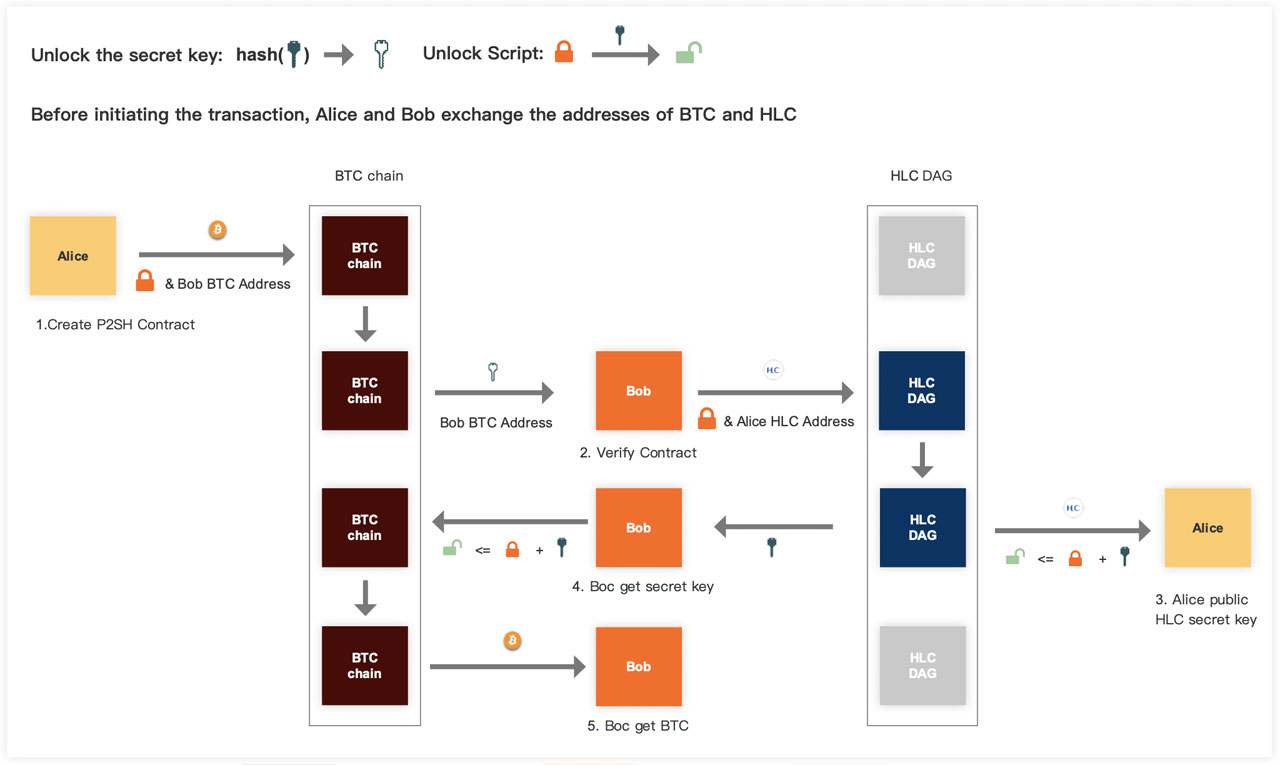
\includegraphics{figures/UTXOAtomicSwap.jpg}}%
	}
\caption{UTXO Atom Swap}
\end{figure}



\subsubsection{Smart Contract Interoperability}

Qitmeer completes the cross- chain transaction between the block chain assets of Qitmeer and  other account models through hash lock Smart contract.

\subsubsection*{Smart Contract Interoperability Process (ETH to MEER)}

\begin{enumerate}
\item  Alice and Bob generate their addresses on 'MEER' and 'ETH' chains respectively;

\item   Alice generates her own \textit{Secret Key} and \textit{Secret Key hash};

 \item  Alice locks her 'MEER' token into the hash-lock contract in the main chain of 'MEER'. The unlocking condition is that Bob holds the \textit{Secret Key} or returns it to Alice after exceeding the specified time;

 \item  Bob checks the contract of Alice in the main chain of 'MEER' and generates the corresponding contract on 'ETH' using \textit{Secret Key hash}. The unlocking condition is that Alice holds the \textit{Secret Key } or returns it to Bob after exceeding the specified time.

 \item  Alice uses \textit{Secret Key} to call Smart Contract to take 'ETH';

 \item  After obtaining \textit{Secret Key}, Bob takes 'MEER' locked by Alice in the hash-lock contract and completes the transaction;

\end{enumerate}


\clearpage
%\appendix
%\section{Appendix}
%\begin{appendices}
%\section{append A}

%Foo bar Foo bar Foo bar Foo bar Foo bar Foo bar Foo bar Foo bar Foo bar Foo bar

%\end{appendices}

%\bibliographystyle{plainnat}
%\bibliographystyle{unsrt,acm}
\bibliographystyle{unsrt}
\bibliography{qitmeer_whitepaper}

\end{document}

